\section{Comparison of {\asas} and {\harps} for period recovery}
\protect\label{section:asasfap}

It seemed appropriate to look in more detail at the {\asas} data which offers similar sampling to that from the {\harps}
data discussed in Section \ref{section:harpsper} above. Of particular importance is the False Alarm Probability of
periods recovered from the spectroscopic data as well as estimating the uncertainty level of all of the calculated
periods, particularly those in the Photometric data. None of the three Python routines directly return an FAP and the
the {\numrecs} routine always returns an FAP of 1 for the periods if the periods were found at all. Consequently a Monte
Carlo method was devised and implemented to study this and at the same time help estimate the uncertainty on the period
obtained from the {\asas} results.

The {\asas} data has many more observations than the spectroscopic data from {\harps}. The former has 970 and the latter
has 316 (or 260 in the Original Set). If the {\asas} data is binned, then as noted in Section \ref{section:asas}, the
number of observations becomes 924 if binned to the most optimal 18 minutes or 624 if binned to 1 day, more akin to the
binning used in many of the periodicity calculations for the {\harps} data, and a more manageable ratio of numbers of
observations.

So, starting from the {\asas} data, binned to 1 day and assuming for the purpose that the 82.6 day period obtained from
the full set as described in Section \ref{section:asas} is correct, various percentage-sized subsets of the data were
randomly selected, recalculating the periods, noting whether a value close to the correct period was recovered as the
strongest peak, within the five strongest peaks, or not at all. If the period was recovered, the RMS error, assessed as
the difference from 82.6 days, was recorded. The sizes of the subsets were taken between 5\% and 95\% in steps of
5\%. For each percentage sized subset, the process was repeated 2,000 times. The results are illustrated in
Fig. \ref{fig:asasprop}.

In Fig. \ref{fig:asasprop} is shown four results. In all cases the X-axis displays the percentage sized subset of the
binned {\asas} data which was used. On the left Y-axis is shown the percentage of recovery (i.e. 100\% minus the FAP) of
the correct period. The blue line shows the percentage recovery of the correct period as the strongest peak with various
percentage sized subsets of the data and the green line shows the percentage recovery of the correct period as one of
the five strongest peaks, not necessarily as the strongest peak. If can be seen that former reaches 100\% recovery at
about 70\% and the latter at about 45\%.

On the right Y-axis is shown the RMS error in the period when it is correctly-recovered period. The purple line shows
the RMS error in the results corresponding to the case where the correct period is recovered as the strongest peak and
the red line the RMS error in the results corresponding to the case where the correct result is found in one of the top
five peaks. It is noticeable that this reaches less than 0.1 days in both cases, lending weight to the conclusion that
the uncertainty in the 82.6 peak found by {\asas} and {\hst} is of the order of 0.1 days at worst.

Finally, marked in as the dotted vertical black lines are the percentages where various numbers of observations with
various clippings and binnings of the {\harps} data would come. The actual numbers of observations range from 55, or
8.8\% of 624, to 316, or 50.6\% of 624. The intersections with the blue lines would indicate the level of FAP which
would be expected from the most powerful peak in the corresponding periodogram and that with the green lines would
indicate the level of FAP as one of the top five peaks. This can be considered alongside the summary in Table
\ref{table:perftable} but that is a condensation of the results in Appendix \ref{chapter:pgramdetail}, some of which
have a larger number of observations than others. It is clear that the best view of the performance from the
spectroscopic methods -- 53\% of the results for Peak Ratio, accepting periods within 2\% is poorer, both in terms of
rate of recovery and in error bar, than could be explained by restriction of the points alone - i.e. about 70\%.

\begin{figure}[!htbp]
\begin{center}
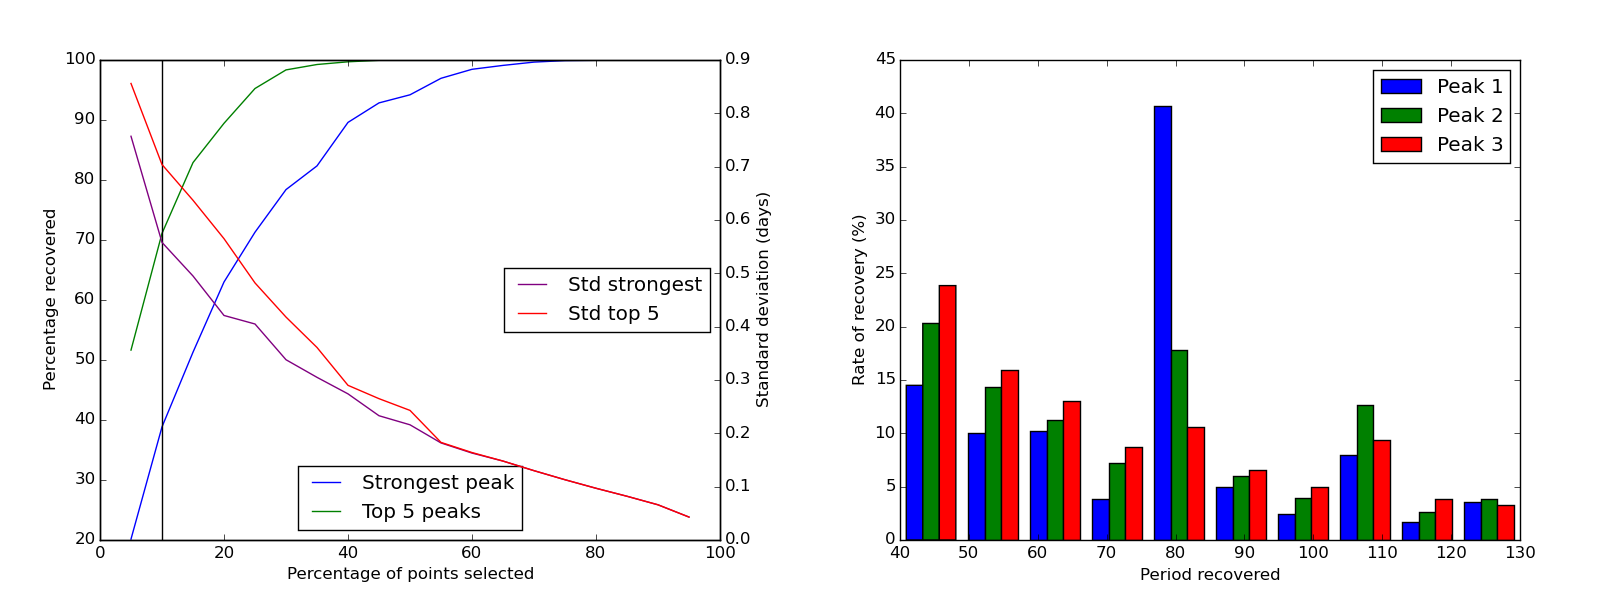
\includegraphics[scale=0.4]{Figures/prop.png} \\
\end{center}   
\caption{In this figure is illustrated the effects of randomly selecting a given proportion of the {\asas} data in terms
  of whether the same period of 82.6 days is recovered and the error in this result. The black vertical dotted lines
  mark in the proportions of data corresponding to the number of observations in the various clippings and binnings of
  the data listed in Table \ref{table:origewtaball} and Table \ref{table:fullewtaball}.}
\protect\label{fig:asasprop}
\end{figure}
